\section{Zielsetzung}
Im Versuch soll die Wärmeleitfähigkeit von Aluminium, Messing und Edelstahl untersucht werden.

\section{Theorie}
Herrscht in einem Körper ein Temperaturungleichgewicht, so wird dieses mittels Wärmetransport
ausgeglichen. Dieser kann auf drei Arten stattfinden. Durch Konvektion, den Wärmetransport
makroskopischer Teilchen, durch Wärmestrahlung, den Wärmetransport mittels elektromagnetischer
Wellen und mittels Wärmeleitung, wobei die Wärme unter anderem über frei bewegliche Elektronen
und nicht durch makrsokopische Teilchenbewegung, weitergegeben wird.
Letzters wird im folgenden Versuch untersucht.
Dazu wird ein Stab der Länge $L$ mit Querschnittsfläche $A$, der Dichte $\rho$, der spezifischen
Wärme $c$ und der materialabhängigen Wärmeleitfähigkeit $\kappa$ betrachtet.
Die Wärmemenge $dQ$, die pro Zeit $dt$ transportiert wird, kann mittels folngenden
Zusammenhangs beschrieben werden:
\begin{equation*}
  \frac{dQ}{dt} = - \kappa A \frac{\partial T}{\partial x} .
\end{equation*}
Das Minuszeichen bedeutete, dass die Wärme vom kälteren, zum wärmeren Teil des Stabes fließt.
Die Wärmestromdichte beträgt folglich:
\begin{equation*}
  j_\symup{w} = - \kappa \frac{\partial T}{\partial x}
\end{equation*}
und mit Hilfe der Kontinuitätsgleichung folgt daraus die eindimensionale Wärmeleitungsgleichung:
\begin{equation*}
  \frac{\partial T}{\partial t} = \frac{\kappa}{\rho c} \frac{\partial^2 T}{\partial x^2}.
\end{equation*}
Die Größe $\sigma_\symup{T} = \frac{\kappa}{\rho c}$ beschreibt dabei, wie schnell sich
der Temperaturunterschied wieder ausgleicht und wird als Temperaturleitfähigkeit bezeichnet.

\noindent Die Temperaturwelle, die sich in einem Stab ausbreitet, welcher periodisch
erhitzt und abgekühlt wird, kann mit folgender Gleichung beschrieben werden:
\begin{equation*}
  T(x, t) = T_\symup{max} exp\left(- \sqrt{\frac{\omega \rho c}{2 \kappa}}x\right) cos \left(\omega t - \sqrt{\frac{\omega \rho c}{2 \kappa}} x\right),
\end{equation*}
die sich mit der Phasengeschwindigkeit
\begin{equation*}
  \nu = \sqrt{\frac{2 \omega \kappa}{\rho c}}
\end{equation*}
ausbreitet.
\FloatBarrier
Die Dämpfung wird aus dem Verhältnis zweier Amplituden$A_\symup{nah}$ und $A_\symup{fern}$
an zwei auseinanderliegenden Messstellen $x_\symup{nah}$ und $x_\symup{fern}$, zueinander bestimmt.
Wird außerdem
\begin{align*}
  \omega = \frac{2 \pi}{T^*} &&&& \Phi = \frac{2\pi \Delta t}{T^*}
\end{align*}
, mit $T^*$ für die Periodendauer der Phase $\Phi$ benutzt, so ergibt sich für die Wärmeleitfähigkeit:
\begin{equation*}
  \kappa = \frac{\rho c (\Delta x)^2}{2 \Delta t \ln{(A_\symup{nah} / A_\symup{fern})}}.
\end{equation*}
$\Delta x$ ist die Entfernung der beiden Messtellen und $\Delta t$ die Phasendifferenz
der Temperaturwelle an den beiden Messstellen.

\section{Durchführung}
Abbildung \ref{abb1} zeigt den Versuchsaufbau.
Die vier Stäbe sind zweimal Messing, und jeweils einmal Aluminium und Edelstahl.
Das Peltier Element dient dabei zum Erhitzen oder Abkühlen der Stäbe, je nach Schaltereinstellung.
Zu Beginn werden die Abstände $\Delta x$ zwischen den Thermoelementen gemessen und
das Netz- und Messgerät angeschlossen. Es ist darauf zu achten, dass die Stäbe während
jeder der Messungen isoliert sind, sodass der Wärmeaustausch mit der Umgebung möglichst gering
gehalten wird.

\begin{figure}
  \centering
  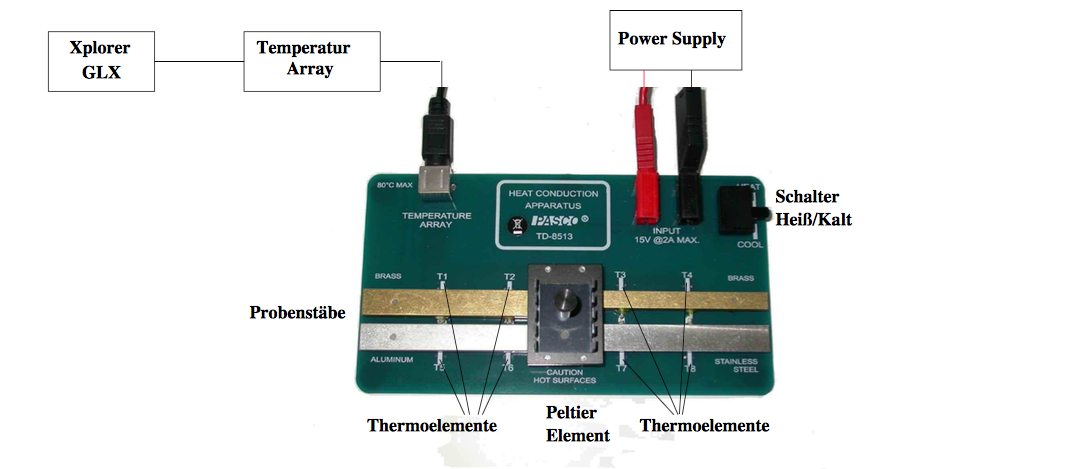
\includegraphics[scale=0.4]{Aufbau.PNG}
  \caption{Versuchsaufbau \cite{Quelle}}
  \label{abb1}
\end{figure}

\subsection{statische Methode}
Zur Durchführung der statischen Methode wird die Spannung des Netzgeräts auf $\SI{8}{\volt}$ und die
Abtastrate des Messgeräts auf $\SI{5}{\per \second}$ eingestellt. Der Schalter am Peltier Element wird
nun auf "Heat" gestellt, sodass sich die Stäbe erwärmen. Hat der Edelstahlstab eine Temperatur
von $\SI{45}{\degree}$ erreicht, so werden anschließend alle Stäbe auf $\SI{30}{\degree}$ abgekühlt
und die Messwerte exportiert.

\subsection{dynamische Mehode}
Bei der dynamischen Methode, wird eine Spannung am Netzgerät von $\SI{11}{\volt}$ und
eine Abtastrate von $\SI{2}{\second}$ benötigt. Dann werden alle vier Stäbe alternierend
für $\SI{40}{\second}$ erhitzt und abgekühlt. Dies wird für 12 Perioden durchgeführt.
Abermals werden die Messwerte exportiert und die Stäbe auf $\SI{30}{\degree}$
abgekühlt. Anschließend folgt analog der zweite Durchgang, in dem die Stäbe jeweils für
$\SI{100}{\second}$ alternieren erhitzt und abgekühlt werden, die Messwerte gespeichert und exportiert werden.

\newpage
\nocite{*}
\printbibliography
